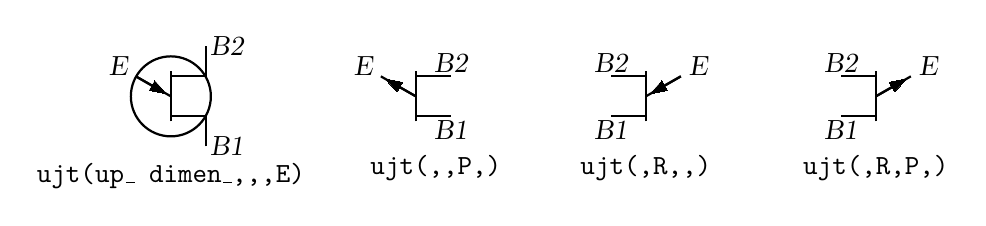
\begin{tikzpicture}[scale=2.54]
% dpic version 2020.03.01 option -g for TikZ and PGF 1.01
\ifx\dpiclw\undefined\newdimen\dpiclw\fi
\global\def\dpicdraw{\draw[line width=\dpiclw]}
\global\def\dpicstop{;}
\dpiclw=0.8bp
\dpiclw=0.8bp
\dpicdraw (0.9,-0.15)
 --(0.9,0)\dpicstop
\dpicdraw (0.9,0)
 --(0.725,0)\dpicstop
\dpicdraw (0.725,-0.025)
 --(0.725,0.225)\dpicstop
\dpicdraw (0.725,0.2)
 --(0.9,0.2)
 --(0.9,0.35)\dpicstop
\dpicdraw (0.55,0.2)
 --(0.725,0.1)\dpicstop
\filldraw[line width=0bp](0.61699,0.129727)
 --(0.703125,0.1125)
 --(0.644553,0.177963) --cycle\dpicstop
\dpicdraw (0.55,0.2)
 --(0.687872,0.121216)\dpicstop
\dpicdraw (0.725,0.1) circle (0.07874in)\dpicstop
\draw (0.9,-0.15) node[right=-2bp]{\sl B1};
\draw (0.4625,0.25) node{{\sl E}};
\draw (0.9,0.35) node[right=-2bp]{\sl B2};
\draw (0.725,-0.3) node{{\tt ujt(up\_ dimen\_,{,},E)}};
\dpicdraw (2.125,0)
 --(1.95,0)\dpicstop
\dpicdraw (1.95,-0.025)
 --(1.95,0.225)\dpicstop
\dpicdraw (1.95,0.2)
 --(2.125,0.2)\dpicstop
\dpicdraw (1.775,0.2)
 --(1.95,0.1)\dpicstop
\filldraw[line width=0bp](1.88301,0.170273)
 --(1.796875,0.1875)
 --(1.855447,0.122037) --cycle\dpicstop
\dpicdraw (1.95,0.1)
 --(1.812128,0.178784)\dpicstop
\draw (2.125,0) node[below=-2bp]{\sl B1};
\draw (1.6875,0.25) node{{\sl E}};
\draw (2.125,0.2) node[above=-2bp]{\sl B2};
\draw (2.05,-0.175) node[below=-2bp]{{\tt ujt(,{,}P,)}};
\dpicdraw (2.925,0)
 --(3.1,0)\dpicstop
\dpicdraw (3.1,-0.025)
 --(3.1,0.225)\dpicstop
\dpicdraw (3.1,0.2)
 --(2.925,0.2)\dpicstop
\dpicdraw (3.275,0.2)
 --(3.1,0.1)\dpicstop
\filldraw[line width=0bp](3.180447,0.177963)
 --(3.121875,0.1125)
 --(3.20801,0.129727) --cycle\dpicstop
\dpicdraw (3.275,0.2)
 --(3.137128,0.121216)\dpicstop
\draw (2.925,0) node[below=-2bp]{\sl B1};
\draw (3.3625,0.25) node{{\sl E}};
\draw (2.925,0.2) node[above=-2bp]{\sl B2};
\draw (3.1,-0.175) node[below=-2bp]{{\tt ujt(,R,{,})}};
\dpicdraw (4.075,0)
 --(4.25,0)\dpicstop
\dpicdraw (4.25,-0.025)
 --(4.25,0.225)\dpicstop
\dpicdraw (4.25,0.2)
 --(4.075,0.2)\dpicstop
\dpicdraw (4.425,0.2)
 --(4.25,0.1)\dpicstop
\filldraw[line width=0bp](4.344553,0.122037)
 --(4.403125,0.1875)
 --(4.31699,0.170273) --cycle\dpicstop
\dpicdraw (4.25,0.1)
 --(4.387872,0.178784)\dpicstop
\draw (4.075,0) node[below=-2bp]{\sl B1};
\draw (4.5125,0.25) node{{\sl E}};
\draw (4.075,0.2) node[above=-2bp]{\sl B2};
\draw (4.25,-0.175) node[below=-2bp]{{\tt ujt(,R,P,)}};
\end{tikzpicture}
\vspace*{-0.5\baselineskip}
